\section{Overall Design of REACH}

\begin{figure}[h]
\fbox{
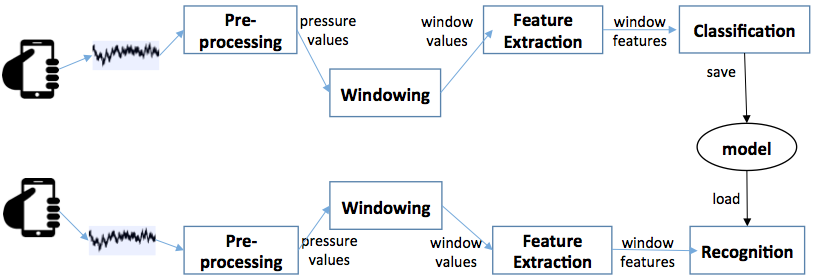
\includegraphics[width=.45\textwidth]{Block_Design_ahmad.png}
}
\caption{Design of REACH}
\label{fig:Design of REACH}
\end{figure}

The design of REACH involves three distinct phases - building the hardware to collect and transmit force sensor data, performing off-line analysis to train a classification model and finally performing real-time evaluations to detect grip patterns and perform a corresponding action. The overall design of REACH is illustrated in Figure \ref{fig:Design of REACH}.
\par
The built-in force sensors continuously send force values to the classification phase of the system. In classification phase, the force values are windowed and suitable features from the window values are extracted. These features are then used to find a suitable classification model and the parameters of the model are saved. In recognition phase, the saved classification model is used to detect the corresponding actions on the phone. We describe each phase of REACH in details in the following sections.

